\documentclass{article}
\usepackage{graphicx}

\begin{document}

\title{11791 - Homework 1 - Named Entity Recognition Implementation with UIMA SDK}
\author{Mohammad Gowayyed \\ mgowayye@andrew.cmu.edu}

\maketitle
\begin{abstract}
In this document, I report briefly my implementation for a gene named entity recognition. I used the algorithm described in \cite{banner} and used some of the published implementation at \cite{banner_code}. Whenever I use any of their code, I am clearly stating this within my Java code. I use CRF from the Mallet library after extracting token features.
\end{abstract}


\section{System Architecture}

Figure \ref{fram} shows the basic architecture of the system. As in the UIMA tutorial, it is recommended to use Analysis Engines instead of CAS Consumers. I have a collection reader that reads the document. Then a preprocessing annotator that creates Sentence objects. Then the feature extraction annotator, that do tokenization, POS tagging and several other features as described in the next section. Based on whether we run a training or a testing program, we will use either training or testing Analysis Engines.\\

The Banner framework uses Mallet (a machine learning library) for training the CRF. They also extract features within the learning process (using Mallet pipes), which I found not a good design, as it depends ({high coupling}) on the machine learning library used. I preferred to separate the feature extraction from the learning totally.

Benefits of separating the features extraction from the learning:
\begin{enumerate}
\item It reduces coupling between feature extraction and the machine learning library used.
\item It is more modular, as we can replace the feature extractor with another feature extractor without needing to change the learning algorithm. Also, we can use a completely other library for learning or another algorithm from the same library without worrying to edit the feature extraction annotator.
\item It is more reusable, as we can use the same exact annotator for both training and testing.
\end{enumerate}
\begin{figure}[h!]
\label{fram} 
\centering
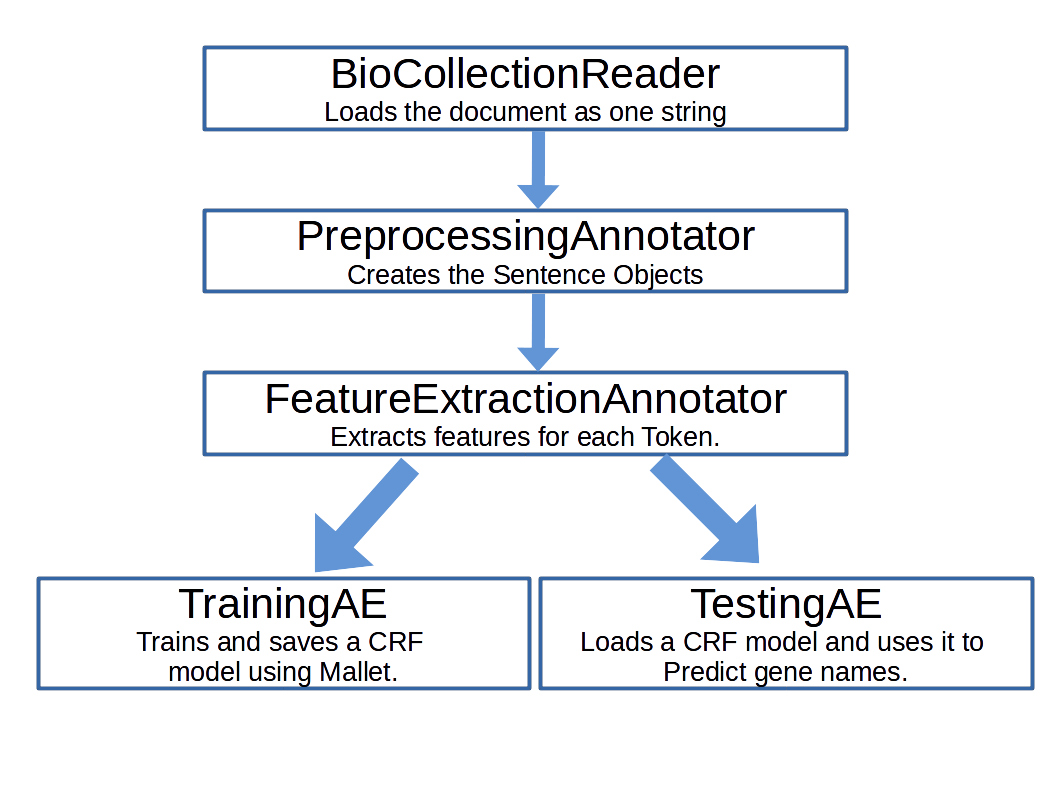
\includegraphics[width=14cm]{framework.png}
  \caption{The general architecture of the system.}
\end{figure}

\begin{figure}[h!]
  \centering
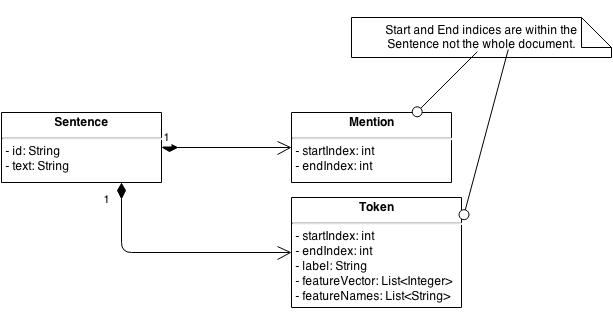
\includegraphics[width=14cm]{HW1-genes-UML.png}

  \caption{A simple class diagram for the Type System I used. The sentence represents a line of the input and the Token is a token in the Sentence. A Mention represents a gene mention.}
\end{figure}


\section{Data Flow and Algorithm}
\subsection{Data Flow}
\subsubsection{BioCollectionReader}
This collection reader loads a whole text document and stores its contents in the JCas document text.\\
\textbf{Input:} The path of the file to load the data.\\
\textbf{Output:} One JCas object with the whole document text.


\subsubsection{PreprocessingAnnotator}
This annotator is responsible for creating Sentence objects from the document loaded by BioCollectionReader.\\
\textbf{Input:} JCas with one String representing the whole document.\\
\textbf{Output:} List of Sentence objects, each has an id and text.\\


\subsubsection{FeatureExtractorAnnotator}
This annotator is responsible for extracting the features for each token of the Sentence. It uses StanfordCoreNLP classes to 1) tokenize 2) get POS tags. It also extracts other features the same as BANNER \cite{banner_code} system does: Regular Expression features and other linguistic features.\\
 
This annotator is generic to work with either training or testing. It is also independent from the learning algorithm and independent from the learning library. In contrast to the BANNER library in which both feature extraction and learning are done using the Mallet library, I separated feature extraction from learning for a better design, so that I have the ability to compare the performance when using different learning algorithms or even different libraries without needing to change my feature extraction annotator.\\
\textbf{Input:} JCas with List of Sentence objects.\\
\textbf{Output:} List of Sentence objects, each has list of tokens and each token has list of feature values.\\




\subsubsection{TrainingAnnotator}
\footnote{TrainingAnnotator and TestingAnnotator should not have been named Annotators as they are not annotators, they work as CAS consumers. I didn't have time to update them in code and tests everything again. As recommended from the UIMA tutorial, I used Analysis Engines instead of CAS consumers.}
This analysis engine is responsible for training a CRF model using Mallet library and stores the model to a file.\\
\textbf{Input:} JCas with List of Sentence objects, each has list of tokens and each token has list of feature values.\\
\textbf{Output:} CRF model file trained using the features extracted in the previous step.\\

\subsubsection{TestingAnnotator}
 This analysis engine is responsible for loading a CRF model and using it to predict gene names, then evaluate the predictions and saves them to an output file.\\
\textbf{Input:} JCas with List of Sentence objects, each has list of tokens and each token has list of feature values.\\
\textbf{Output:} Detected gene names in an output file and F1-score calculated and printed to the console.\\


\subsection{Algorithm}
BANNER \cite{banner} uses Conditional Random Fields (CRF), which assigns a probability distribution for the labels of each token. First the sentence text is tokenized, then for each token they extract features: POS, Lemmatization, and several RegEx features\footnote{find their details in ae.FeatureExtractorAnnotator::addRegExFeatures}. Then they train a CRF model using these features.\\

For testing the CRF model provides the label that has the highest probability for each Token.
\section{Experiments}

I used the \textit{sample.in} and \textit{sample.out} files to train and test the model. I gradually added features to make sure that more features is reflected into an increase in the F1-score.\\

When training using only the words as features, I got \textbf{0.366} F1-score. Adding POS tagger increased the F1-score to become \textbf{0.702}. After adding regular expression features (find their details in ae.FeatureExtractorAnnotator::addRegExFeatures), my final F1-score became \textbf{0.893}.

\subsection{If you failed to run my code}
Check the paths at \textit{Config} class, if the problem is in the paths.

\begin{thebibliography}{9}


\bibitem{banner}
BANNER: an executable survey of advances in biomedical named entity recognition,
Leaman, Robert and Gonzalez, Graciela and others,
  Pacific Symposium on Biocomputing,
  2008

\bibitem{banner_code}
  http://banner.sourceforge.net/

\end{thebibliography}
\end{document}